\chapter{Introduction to JuPE}

Optimization problems can be in the broadest sense described as problems where an optimal solution is obtained using a limited amount of resources. Many problems that exist in the field of engineering and natural science can be categorized as optimization problems. For example, when mapping applications are used to navigate between two points, an algorithm tries to find the shortest path to a destination by choosing the direction of travel while under constraints such as traffic laws or avoiding road work.
Gradient-based iterative algorithms are a prominant tool to solve large optimization problems. Their ability to efficiently optimize functions without requiring an explicit formula means they are extensively used in fields such as machine learning and data science. As the term encompasses many algorithms, each can solve any of the many types of optimization problems with varying levels of speed and accuracy, making it very useful the ability to compare algorithms on specified metrics and identifying the one best suited for a problem. But while these algorithms are widely, their analysis have only been available to those with an in depth knowledge of the underlying math until recently \cite{pepit}. The main work of this thesis presents a tool for analysis of gradient-based algorithms' performance characteristics accessible to non-experts.

JuPE (Julia Performance Estimation) is a computer program written in the Julia programming language that automatically and systemically finds the worst-case performance guarantee of an algorithm at solving a specified set of problem. After the program is given a class of functions, the algorithm to be analyzed and the performance metrics, it returns a guarantee speed at which the algorithm inputted can solve any function in the provided set.


%%%%%%%%%%%%%%%%%%%%%%%%%%%%%%%%%%%%%%%%%%%%%%%%%%%%%%%%%%%%%%%%%%%%%%%%%%%%%%%%
\section{Optimization problems and algorithms}

In this paper, the optimization problem considered is in the form of finding the minimum point of a continuously differentiable function:
\begin{subequations}\label{opt prob}
  \begin{align}
    \textrm{minimize} \quad f(x) \\
    \textrm{subject to} \quad x \in X
  \end{align}
\end{subequations}
Where \(f(x)\) is the optimization function and \(X\) is a constraint set. Here, \(x\) is the input and \(f(x)\) is a measure of how close a solution is to being optimal. Well-known examples of this problem are large language models (LLMs) such as ChatGPT and machine learning models that enable self-driving features in automotives, amongst many others. These models are only possible due to the minimizing of loss functions, a fundamental part of their training where a function is used to quantify the dissimilarity between a model's output and the target values, and the model's parameters are modified iteratively in order to minimize the function and improve the model's performance.

While traversing any function can give its minimum, for large-scale and complex problems, it is more efficient to be optimize numerically using iterative gradient-based  algorithms. These algorithms minimize a function by starting at an initial point \(x_{0}\) and iteratively updating \(x_k\) (\(k\) representing the current iteration number) using the gradient of the function at the last iteration $\nabla$ \(f(x_k)\) until it reaches a local minimum \(x_*\). For example, the gradient descent (GD) algorithm updates \(x_k\) following this formula:
\begin{equation}\label{eqn:GD}
  x_{k+1}=x_{k}-\alpha \nabla f(x_k)
\end{equation}
Where $\alpha$ is the step size, an adjustable parameter of the algorithm. $\alpha$ can affect the speed at which the algorithm converges, or whether it converges at all, in which case overshooting occurs. Following this update formula, in each iteration, \(x\) moves toward the goal \(x_*\). Accelerated algorithms exist that seek to solve the problem of overshooting, such as Polyak’s Heavy Ball (HB) method which introduces a momentum that incorporates previous iterations of \(x\):
\begin{equation}\label{eqn:HB}
  x_{k+1}=x_k-\alpha \nabla f(x_k)+ \beta (x_k-x_{k-1})
\end{equation}
While Nesterov’s Fast Gradient (FG) evaluates the gradient at an interpolated point:
\begin{subequations} \label{eqn:FG}
  \begin{align}
    x_{k+1}     &=x_k-\alpha \nabla f(y_k), \label{eq_state}       \\
    y_{k+1} &=x_{k+1}+\beta (x_{k+1}-x_k) \label{eq_interpolated point}
  \end{align}
  \end{subequations}
%%%%%%%%%%%%%%%%%%%%%%%%%%%%%%%%%%%%%%%%%%%%%%%%%%%%%%%%%%%%%%%%%%%%%%%%%%%%%%%%
\section{Algorithm analysis}
Let us consider the problem of minimizing a simple quadratic function:
\begin{equation} \label{eqn:quadratic}
    f(x) = x^2/2 - 3x + 4
\end{equation}

Using (GD) equation \ref{eqn:GD}, substituting step size $\alpha$ with values 0.2, 0.5, and 2, and picking a starting point of $x_0 = 0$, we can solve the quadratic function. By counting the number of iterations each variation runs for before reaching 0.001 of the true minimum, we can measure the iteration complexity:

\begin{figure}[htp]
  \centering
  \begin{subfigure}{.5\textwidth}
    \centering
    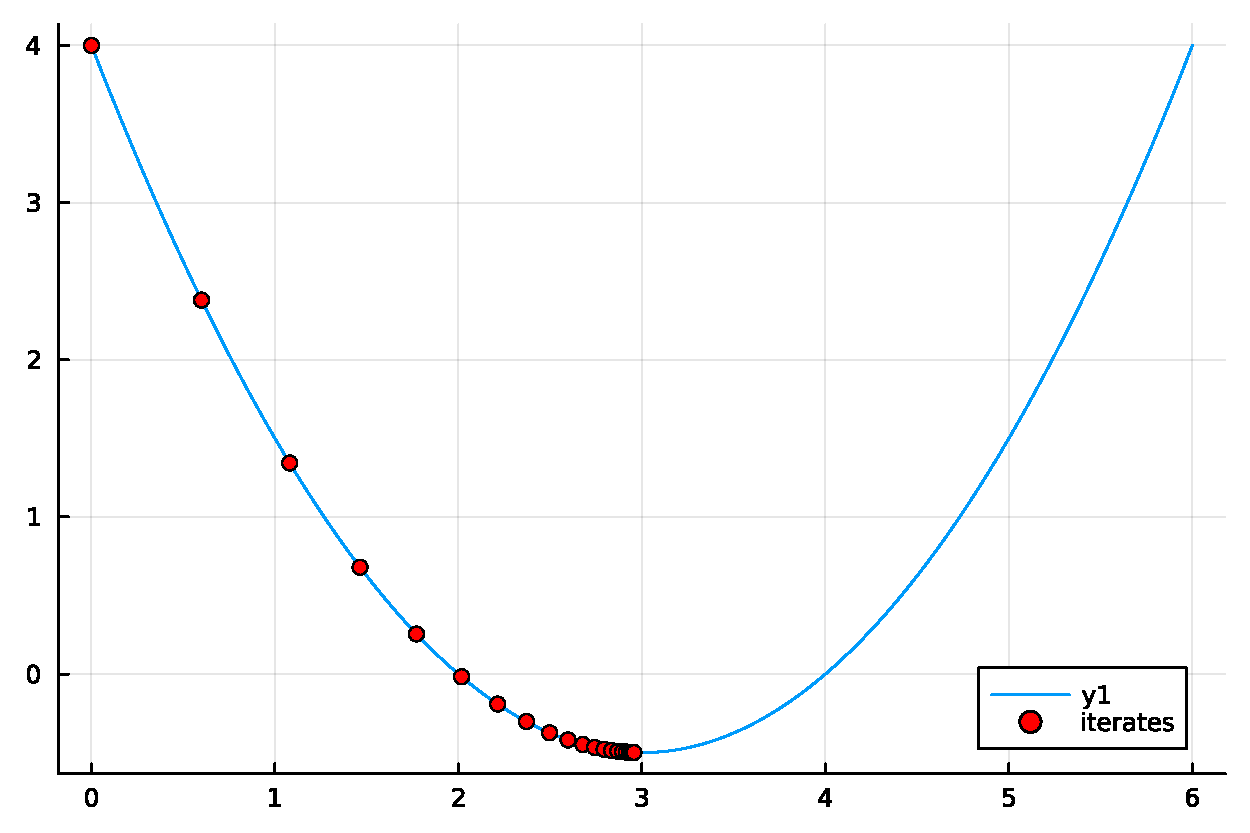
\includegraphics[width=.9 \linewidth]{crude1}
    \caption{$\alpha = 0.2$, iteration complexity = 20}
    \label{fig:crude1}
  \end{subfigure}%
  \begin{subfigure}{.5\textwidth}
    \centering
    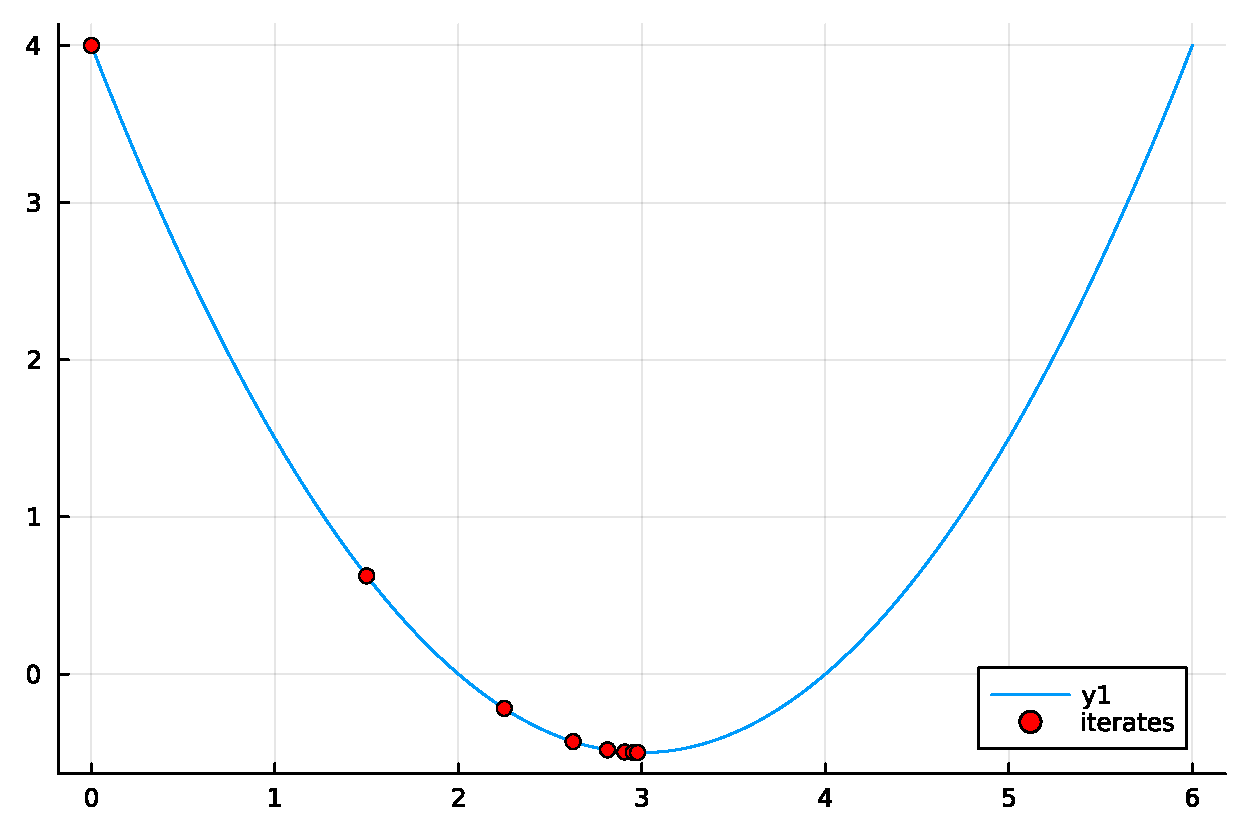
\includegraphics[width=.9 \linewidth]{crude2 }
    \caption{$\alpha = 0.5$, iteration complexity = 7}
    \label{fig:crude2}
  \end{subfigure}
  \begin{subfigure}{.5\textwidth}
    \centering
    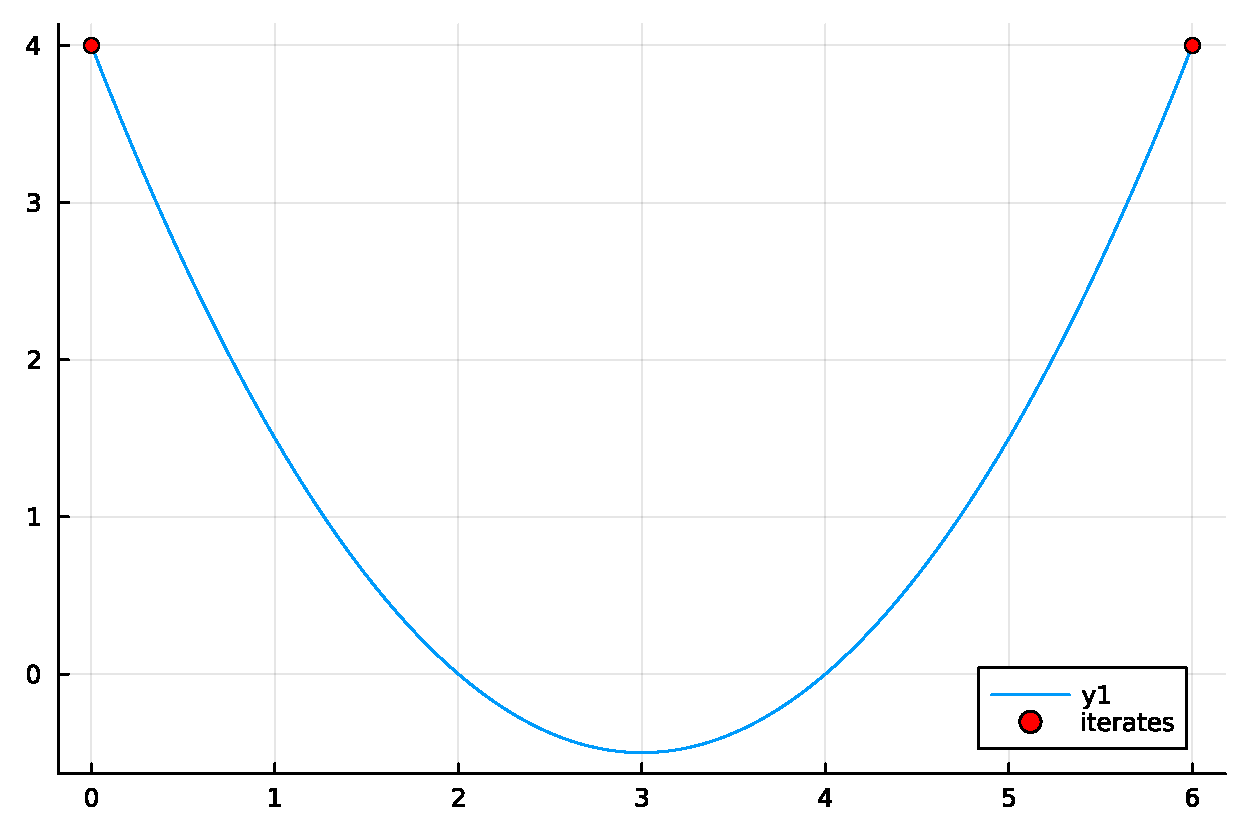
\includegraphics[width=.9 \linewidth]{crude3 }
    \caption{$\alpha = 2$, does not converge}
    \label{fig:crude3}
  \end{subfigure}
  \caption{Performance of 3 GD variants of different step sizes}
\label{fig:test}
\end{figure}

% \begin{figure}[htp]
%   \centering
%   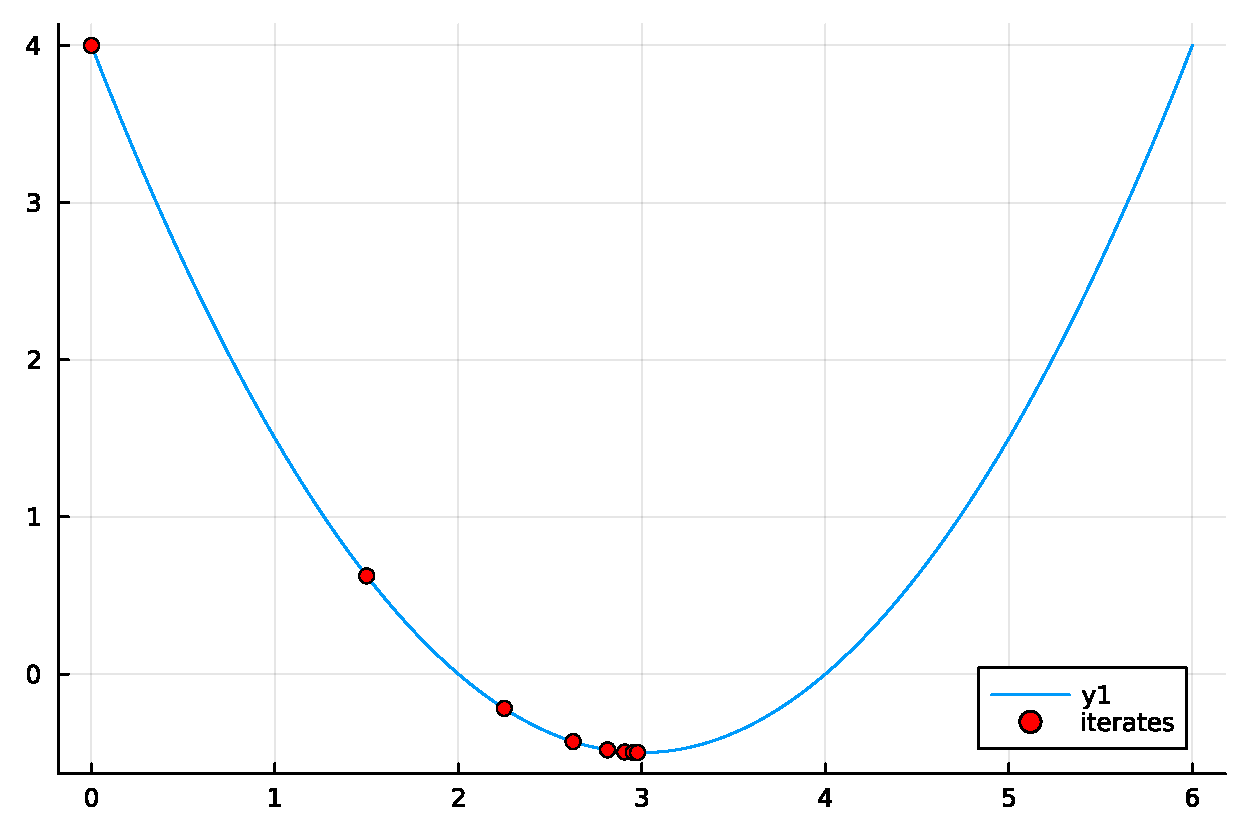
\includegraphics[width=.6\textwidth]{crude2}\hfill
%   \caption{$\alpha = 0.5$, iteration complexity = 21}
%   \label{fig:crude2}
% \end{figure}
% \begin{figure}[htp]
%   \centering
%   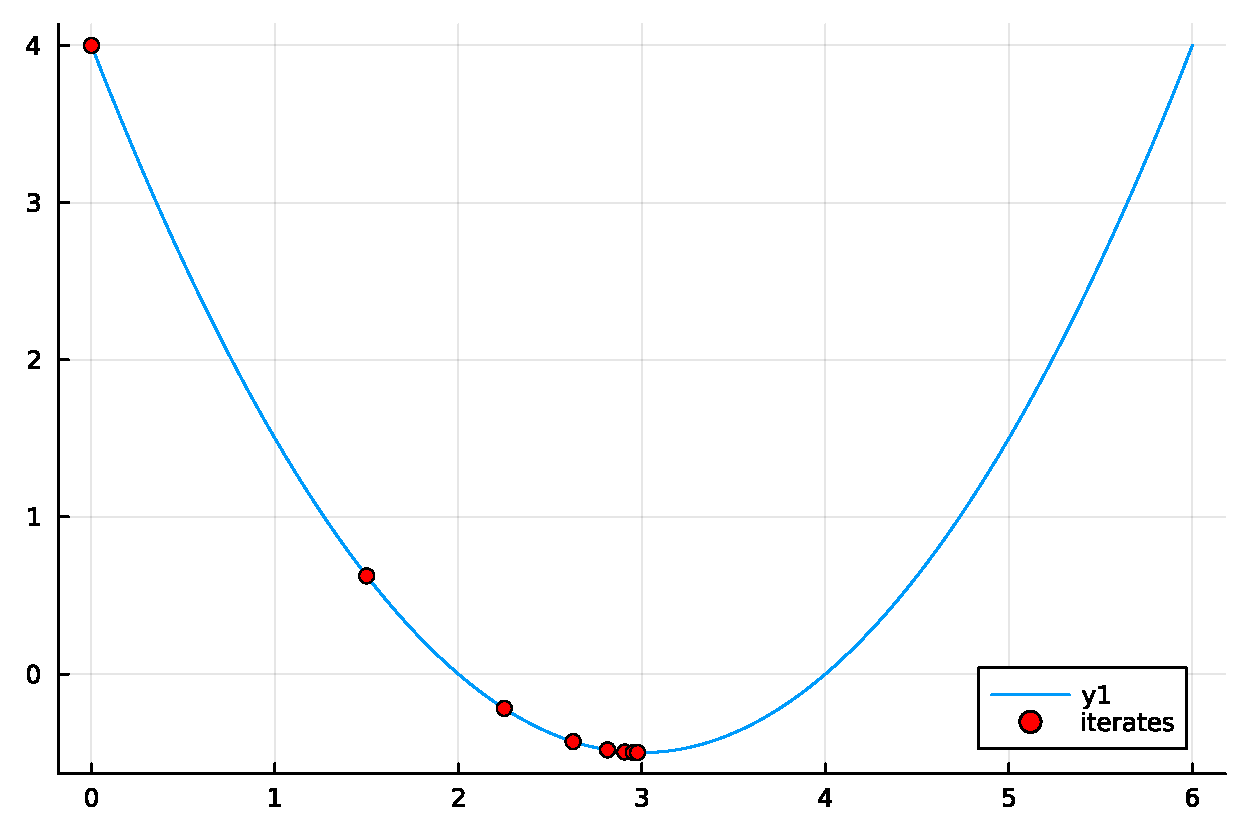
\includegraphics[width=.6\textwidth]{crude2}\hfill
%   \caption{$\alpha = 2$, does not converge}
%   \label{fig:crude3}
% \end{figure}

It can be seen how different tunings on the same algorithm can achieve drastically different speed optimizing a function, or whether it can solve for the minimum at all. Considering there exist many other first order methods in addition to the three in 1.1, each infinitely adjustable by changing the step size or by changing the number of past iterations used, being able to predict how an algorithm will perform before solving an optimization problem can mean a more accurate solution can be found and in fewer iterations. And while the example is of a simple function where overshoot in the case of the third tuning can easily be identified, and the number of iteration needed is small, the benefit of using an optimal algorithm only increases as the problem gets bigger and more complex. Using the same example of training large language and self-driving models, the training process has been and might need to go on for years as more training data is available and the models need to continously improve all while using vast amounts of computational power. As a result, even a small improvement in the performance of the algorithm used can lead to large savings in time and energy.

Considering the quadratic function example, while it yielded an analysis of the algorithms' performance, it required solving the optimization problem. Not only would solving any problem large enough to warrant being optimized numerically in the first place computationally expensive, any benefit of finding a superior algorithm at solving a problem is negated as said problem has already been solved. Additionally, any analysis result is applicable only to one function and cannot be reliably used to derive a first-order method's performance on any other problem.

Due to these limitations, it is more efficient to analyze algorithms' performance at solving a broader set of problem. As a result of their widespread application, popular iterative gradient-based algorithms have been extensively analyzed, a frequently cited example being \cite{adam}. In this paper, the author designed and conducted experiments where how the algorithms perform in typical applications is recorded. While this approach is can provide a general evaluation of an algorithm's performance, it is done emperically. Instead, there exists approaches toward analyzing algorithms \cite{drori2012}, \cite{taylor2016}, and \cite{lessard2016} that aim to find a mathematically provable performance guarantee of an algorithm over a class of functions. This worst-case analysis is referred to as algorithm analysis: Given that a characteristic that a set of functions might share (such as being convex or quadratic), algorithm analysis would return the worst-case performance measure that guarantee the algorithm analyzed would perform as good or better solving every function within said set.

\section{Julia programming language}

JuPE is written in the Julia programming language, a high-level programming language designed specifically for high-performance numerical computing. Julia's compiler performance has been benchmarked to be faster than many other languages used for numerical computing while rivalling C, a language often used for its high efficiency \cite{julia}. Julia accomplishes this while being a high-level language with simple syntax rules that resembles existing popular languages, making it easy to code with and to understand.

Julia was also chosen as it is designed for numerical computing, supporting matrices as well as UTF-8 encoding, making it possible to use scientific notation: variables and functions as they exist in the code and as the user inputs them into the program can use math symbols or Greek letters. This makes Julia excel at communicating mathematical concepts, which simplifies both the process of coding the program and understanding its mathematical underpinnings.

Julia was also chosen as it is open-source and available for free. As JuPE is a package designed for expert and novice users alike to install and use, it made sense to choose Julia as it available on many of the popular platforms such as macOS, Windows, and Linux.

\section{Overview}

JuPE performs worst-case algorithm analysis when three main inputs are provided: The class of functions in question, the algorithm being analyzed, and a performance measure. The package then performs the algorithm analysis and returns the fastest guaranteed convergence rate.

Users can pick from one of the algorithms provided in the package or create their own iterative first-order algorithm by specifying how it is updated. The class of functions can be provided by detailing the characteristic of the set, such as 1 strong 10 smooth convex function. Users can specify a performance measure, which can be how far the iterate \(x_k\) is from the goal \(x_*\) or any quadratic combinations of the iterates. Throughout the process, the user never has to change the code of the package or understand how JuPE works, making it an easy to use black box tool.

In the next chapters, we will 1) discuss the mathematical approach that JuPE utilize, 2) break down the code structure of the program and how it functions, and 3) show some of the analysis that the package has done.